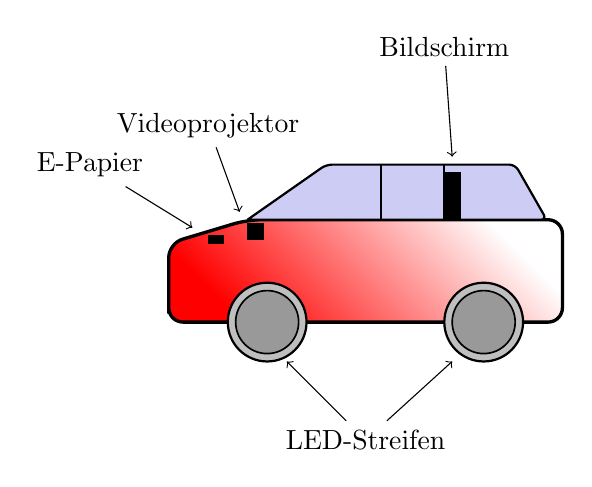
\begin{tikzpicture}
	\shade[top color=red, bottom color=white, shading angle={135}]
	[draw=black,fill=red!20,rounded corners=1.2ex,very thick] (1.5,.5) -- ++(0,1) -- ++(1,0.3) --  ++(3,0) -- ++(1,0) -- ++(0,-1.3) -- (1.5,.5) -- cycle;
	\draw[very thick, rounded corners=0.5ex,fill=black!20!blue!20!white,thick]  (2.5,1.8) -- ++(1,0.7) -- ++(2.4,0) -- ++(0.4,-0.7) -- (2.5,1.8);
	\draw[thick]  (4.2,1.8) -- (4.2,2.5);
	\draw[thick]  (5,1.8) -- (5,2.5);
	\draw[draw=black,fill=gray!50,thick] (2.75,.5) circle (.5);
	\draw[draw=black,fill=gray!50,thick] (5.5,.5) circle (.5);
	\draw[draw=black,fill=gray!80,semithick] (2.75,.5) circle (.4);
	\draw[draw=black,fill=gray!80,semithick] (5.5,.5) circle (.4);
	\node[] (S1) at (0.5, 2.5){E-Papier};
	\node[] (S2) at (4, -1){LED-Streifen};
	\node[] (S3) at (5, 4){Bildschirm};
	\node[] (S4) at (2, 3) {Videoprojektor};
	\draw[fill=black] (2,1.5) -- ++(0.2, 0) -- ++(0, 0.1) -- ++ (-0.2, 0) -- ++(0, -0.1);
	\draw[fill=black] (2.5,1.55) -- ++(0.2, 0) -- ++(0, 0.2) -- ++ (-0.2, 0) -- ++(0, -0.2);
	\draw[fill=black] (5,1.8) -- ++(0.2, 0) -- ++(0, 0.6) -- ++ (-0.2, 0) -- ++(0, -0.6);
	\draw[->] (S1) -- (1.8,1.7);
	\draw[->] (S4) -- (2.4,1.9);
	\draw[->] (S3) -- (5.1,2.6);
	\draw[->] (S2) -- (5.1, 0);
	\draw[->] (S2) -- (3, 0);
\end{tikzpicture}